37. \begin{figure}[ht!]
\center{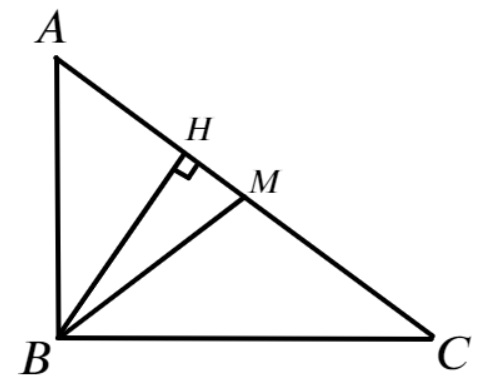
\includegraphics[scale=0.35]{g8-37.png}}
\end{figure}\\
Проведём медиану $BM,$ она равна половине гипотенузы $10:2=5$см. Проведём высоту $BH,$ она либо совпадает с медианой, либо меньше её как катет в прямоугольном треугольнике $BHM.$ Тогда $S=\cfrac{1}{2}\cdot BH\cdot AC\leqslant  \cfrac{1}{2}\cdot BM \cdot AC=\cfrac{1}{2}\cdot 5\cdot 10=25\text{ см}^2.$\\
